% !TEX program = pdflatex
% !TEX options = -synctex=1 -interaction=nonstopmode -file-line-error -shell-escape "%DOC%"
\documentclass{beamer}
\usepackage{graphicx,url}
\usepackage[brazil]{babel}   
\usepackage[utf8]{inputenc}
\usepackage{pgf,tikz}
\usepackage{adjustbox}
\usepackage{mathrsfs}
\usepackage{minted}
\usepackage{listings}
\usetikzlibrary{calc}
\usetikzlibrary{arrows}
\batchmode
\usepackage{amsmath,amssymb,enumerate,epsfig,bbm,calc,color,ifthen,capt-of}
\usetheme{Berlin}
\usetikzlibrary{patterns, matrix, fit, positioning, backgrounds}
\tikzset{square matrix/.style={
    matrix of nodes,
    column sep=-\pgflinewidth, 
    row sep=-\pgflinewidth,
    nodes in empty cells,
    nodes={draw,
      minimum height=#1,
      anchor=center,
      text width=#1,
      align=center,
      inner sep=0pt
    },
    nA/.style={draw, pattern=dots, pattern color=green!70!black},
    nB/.style={draw, pattern=vertical lines, pattern color=blue!70!black},
    nC/.style={draw, pattern=bricks, pattern color=red!80!white},
    nD/.style={draw, pattern=fivepointed stars, pattern color=yellow!80!black},
    nO/.style={draw, fill=black}
  },
     square matrix/.default=0.65cm
}

%-------------------------Titulo/Autores/Orientador------------------------------------------------
\title[Dynamic Programming on Tree]{
  Dynamic Programming on Tree
}
\subtitle {MCPC-2020 Winter Training}
\date{}
\author[Shizhe Zhao (eggeek)]{
  Shizhe Zhao (eggeek)
}

\pgfdeclareimage[height=0.7cm]{monash-logo}{icpc.pdf}
\logo{\pgfuseimage{monash-logo}\hspace*{0.5cm}}

% -----------------------------------------------------------------------------
\begin{document}
% -----------------------------------------------------------------------------

%---Summary---------------------------------------------------------
\frame{\titlepage}

\begin{frame}
  \frametitle{Introduction}
\begin{itemize}
  \item DP is everywhere: contest, industry, research, daily life \ldots
  \item Tree is also everywhere \ldots
  \item DP on Tree is a good start point
\end{itemize}

\end{frame}
\begin{frame}{Tree: definition}
\begin{minipage}{.3\textwidth}
  \begin{figure}[h]
  
\includegraphics[width=.9\textwidth]{pics/tree.png}
  \caption{Unroot tree}
  \end{figure} 
\end{minipage}%
\begin{minipage}{.7\textwidth}
\begin{itemize}
  \item Tree: has 1 (or 0) root
  \item Node: has parent (1 or 0) and children (0 or many)
  \item Root: has 0 parent
  \item Leaf: has 0 child
\end{itemize}
\only<2-> {
\small 
Warm up Question: how many edges in a tree with $n$ nodes?
}

\only<3-> {
  \small
  A: $\mathbf{n-1}$.
}
\end{minipage}
\end{frame}

\begin{frame}
  \frametitle{Tree: examples}
\begin{itemize}
  \item Tree (biological)
  \item File system
  \item Package manger system
  \item and more advance examples \ldots
\end{itemize}
\end{frame}

\begin{frame}
  \frametitle{Tree: examples}
  Search space
  \begin{figure}[]
    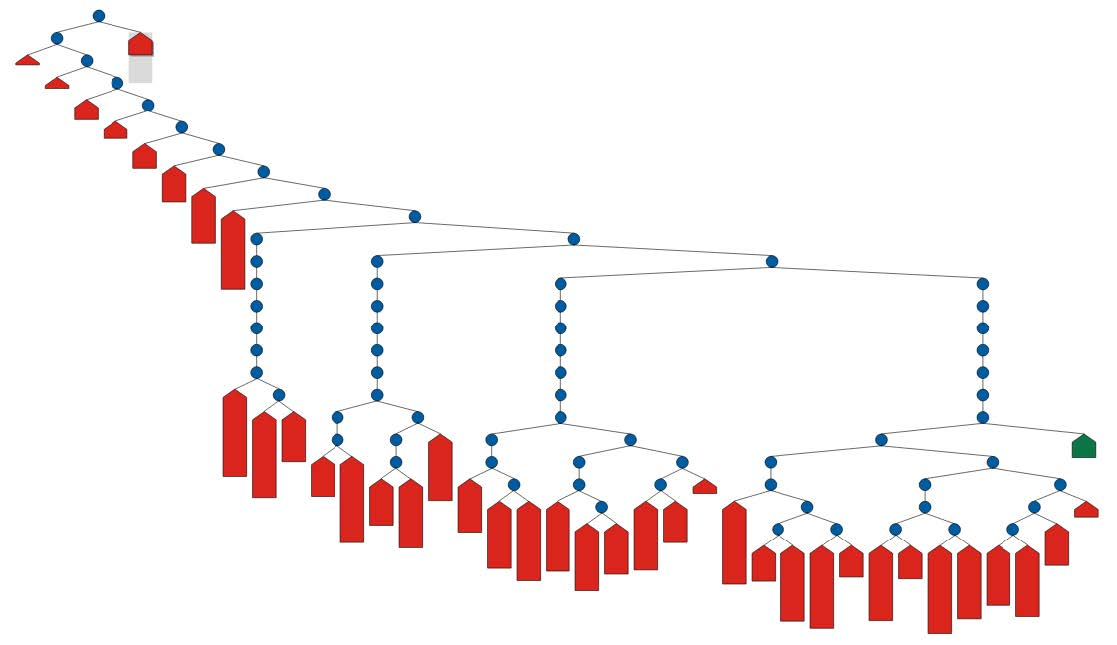
\includegraphics[width=.7\textwidth]{./pics/search-tree.jpg} 
  \end{figure}
  \tiny {Search space of a MiniZinc solver}
\end{frame}

\begin{frame}
  \frametitle{Tree: example}
  \begin{minipage}{.6\textwidth}
    Dijkstra propagation is also a tree
    \begin{itemize}
       \item \textit{Dijkstra}s (on different sources) are not independent
       \item $sp(s_2, m) + sp(m, *) = sp(s_2, *)$
    \end{itemize}
    \end{minipage}%
    \begin{minipage}{.4\textwidth}
     \begin{tikzpicture}
       \matrix[square matrix](lm)
{
    & & |[fill=blue!50]| $*$& |[fill=blue!50]| $*$ \\
    & & |[fill=blue!50]| $m$ & |[fill=blue!50]| $*$ \\
    & |[fill=yellow]| $s_2$ & |[fill=yellow]| $s_1$ & \\
    & & & \\
}; 
    \end{tikzpicture}   
    \end{minipage}
\end{frame}

\begin{frame}
  \frametitle{Tree: diameter}
\begin{definition}
  Diameter of a tree is $\mathbf{max(dist(u, v) | u, v \in Tree)}$
\end{definition}
\begin{minipage}{.3\textwidth}
  \hspace{-3mm} 
  \begin{figure}[]
    
\includegraphics[width=.6\textwidth]{pics/tree.png} 
    \caption{Diameter is $4$}
  \end{figure} 
\end{minipage}%
\begin{minipage}{.7\textwidth}
\only<2-> {Solution:}
\begin{itemize}
  \item<2-> randomly choice a root $u$
  \item<3-> find the furthest node $v$ to $u$
  \item<4-> find the furthest node $w$ to $v$, $dist(w, v)$ is diameter
\end{itemize}  
\end{minipage}
\only<5-> {
  Reasoning: 

  $v$ must be a leaf; and it must be one of the end point on the "diameter path" 
  
  \footnotesize{( hint: proof by contradiction, or \url{http://courses.csail.mit.edu/6.046/fall01/handouts/ps9sol.pdf})}
}

\end{frame}

\begin{frame}
  \frametitle{Dynamic Programming}
  \begin{itemize}
    \item \textbf{Dynamic:} consider the current `status'
    \item \textbf{Programming:} making decision
  \end{itemize}
  \only<2-> {In narrow sense: making decision based on current status to achieve global optimal.}

  \only<3-> {In broad sense: divide and conquer, memorization, combinatorial counting, \ldots}
\end{frame}

\begin{frame}
  \frametitle{Dynamic Programming on Tree}
Classic DP examples: knapsack, coin change \ldots,

they are not friendly to beginners:
\begin{itemize}
  \item context sensitive: any small changes on problem statement (i.e. scenario description) cause a very different model.
  \item abstract: models usually imply a DAG (Directed Acyclic Graph) in multi-dimension
\end{itemize}

while Tree DP is relative easier as the structure is given, and you only need to focus on fit your problem in tree model.
\end{frame}

\begin{frame}
  \frametitle{Dynamic Programming on Tree}
Let's overkill the tree-diameter problem.

Observation: diameter passes through the root or present in any subtree.
\begin{minipage}{.2\textwidth}
\begin{figure}[]
  
\includegraphics[width=.9\textwidth]{pics/tree.png}
\end{figure}
\end{minipage}%
\begin{minipage}{.8\textwidth}
 \begin{itemize}
  \footnotesize
  \item<2-> Randomly choose a root $r$;
  \item<3-> Precompute $L_r[i]$ for each node $i$: the max distance from $i$ to any leaf in it's subtree
  \item<4-> Compute the max distance of path that pass through $r$ ($max(L_{r}[a]+1 + L_{r}[b]+1)_{a, b \in children(r)}$).
  \item<5-> Move the root to an adjacent node $r'$, and regard $r$ as a child of $r'$
  \item<6-> Notice for all nodes under the subtree rooted at $r'$,  $L_{r'}[i]$ is same as previous iteration(i.e. when root is $r$)
  \item<7-> Repeat the 3rd step
\end{itemize} 
\end{minipage}

\end{frame}

\begin{frame}[fragile]
  \frametitle{Static memory location is limited}
Only using static allocated memory can be a bit complicated in some cases:
\begin{itemize}
  \item Store a graph: native way need $O(n^2)$ space
  \begin{minted}[frame=lines]{c++}
  int nodes[N][N];
  \end{minted}
  \item Describe discrete multi-dimension status
  \begin{minted}[frame=lines]{c++}
    // count the number of ways in grid
    if (condition1) cnt[x][y] += cnt[x-1][y];
    if (condition2) cnt[x][y] += cnt[x][y-1];
  \end{minted}
\end{itemize}
\end{frame}

\begin{frame}[fragile]
  \frametitle{Using STL}
  \begin{minted}[linenos=true, frame=lines, fontsize=\footnotesize]{c++}
    // store a graph with at most N nodes
    const int N = 1000;
    vector<int> g[N];
    // dynamically
    vector<vector<int>> g;
    g.resize(n);

    // count the number of ways in grid
    typedef pair<int, int> pii;
    pii status = {x, y};
    map<pii, int> cnt; // like Python dict
    if (condition1) cnt[{x, y}] += cnt[{x-1, y}];
    if (condition2) cnt[{x, y}] += cnt[{x, y-1}];
  \end{minted}
\end{frame}

\begin{frame}[fragile]
  \frametitle{Using STL - example: max \textit{dist} from root to leave}
\begin{minted}[linenos=true, frame=lines, fontsize=\tiny]{c++}
#include <bits/stdc++.h>
using namespace std;
const int N = 1000;
vector<vector<int>> tree;
vector<int> dist;

// call dfs(0, -1) for root=0
void dfs(int cur, int pa) {
  dist[cur] = 0;
  for (auto& it: tree[cur]) if (it != pa) { // recurse to all neighbors except for the parent
    dfs(it, cur);
    dist[cur] = max(dist[cur], dist[it] + 1);
  }
}

void read_tree() {
  int n, u, v;
  cin >> n;
  tree.resize(n); dist.resize(n);
  // tree has exactly n-1 edges
  for (int i=0; i<n-1; i++) {
    cin >> u >> v; 
    // add bidirectional edge
    tree[u].push_back(v); tree[v].push_back(u);
  }
}
\end{minted}
\end{frame}

% -----------------------------------------------------------------------------
\end{document}
%-----------------------------------------------
